\documentclass{standalone}
\usepackage{pgfplots}
\pgfplotsset{compat=1.13}
\usepackage{xcolor}
\begin{document}
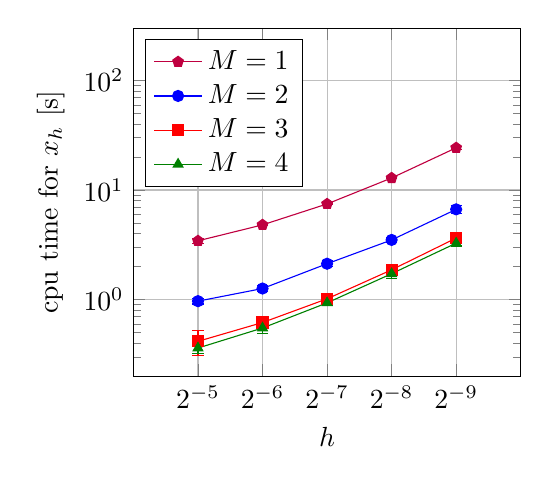
\begin{tikzpicture}
	\begin{semilogyaxis}[
		xlabel= {$h$},
		ylabel={cpu time for $x_h$ [s]},
		xmin = 0,
		xmax = 6,
		xtick = {1,2,3,4,5,6},
		xticklabels = {$2^{-5}$,$2^{-6}$,$2^{-7}$,$2^{-8}$,$2^{-9}$},%$2^{-10}$},
		ymin = 0.2,
		ymax = 300,
		%ytick = {0.001,0.01,0.1,1,10,100},
		xmajorgrids,
		ymajorgrids,
		width=6.5cm,
		height=6cm,
		legend pos=north west,
	]	
	
\addplot+ [purple, mark=pentagon*, mark options={purple},
error bars/.cd,y dir=both,y explicit,
] coordinates {
(1,3.4375) +- (0.1724,0.1724)
(2,4.8063) +- (0.0628,0.0628)
(3,7.4641) +- (0.0834,0.0834)
(4,12.8844) +- (0.1252,0.1252)
(5,24.2875) +- (0.7271,0.7271)
%(6,10.7359) +- (2.5885,2.5885)
};
\addlegendentry{$M = 1$};	
	
\addplot+ [blue, mark=*, mark options={blue},
error bars/.cd,y dir=both,y explicit,
] coordinates {
(1,0.9672) +- (0.0560,0.0560)
(2,1.2609) +- (0.0722,0.0722)
(3,2.1234) +- (0.1321,0.1321)
(4,3.5031) +- (0.1903,0.1903)
(5,6.6609) +- (0.5419,0.5419)
%(6,5.2250) +- (1.3636,1.3636)
};
\addlegendentry{$M = 2$};		
	
\addplot+ [red, mark=square*, mark options={red},
error bars/.cd,y dir=both,y explicit,
] coordinates {
(1,0.4156) +- (0.1085,0.1085)
(2,0.6172) +- (0.0629,0.0629)
(3,1.0156) +- (0.0872,0.0872)
(4,1.8687) +- (0.1217,0.1217)
(5,3.6422) +- (0.1354,0.1354)
%(6,3.4531) +- (0.3255,0.3255)
};
\addlegendentry{$M = 3$};	

\addplot+ [green!50!black,mark=triangle*, mark options={green!50!black},
error bars/.cd,y dir=both,y explicit
] coordinates {
(1,0.3609) +- (0.0374,0.0374)
(2,0.5500) +- (0.0622,0.0622)
(3,0.9328) +- (0.0467,0.0467)
(4,1.7219) +- (0.1773,0.1773)
(5,3.2734) +- (0.1928,0.1928)
%(6,3.4109) +- (1.0184,1.0184)
};
	\addlegendentry{$M = 4$};
	\end{semilogyaxis}
\end{tikzpicture}
\end{document}